\section{Evaluation}
The authors use three different real life time series data and evaluate their results with some existing state of the art data reduction approaches.
The authors use the following datasets:
\begin{enumerate}
	\item the price of a single
	share on the Frankfurt stock exchange over 6 weeks (700k
	tuples)
	\item 71 minutes from a speed sensor of a soccer ball
	\cite{mutschler2013debs}(ball number 8, 7M rows)
	\item one week of sensor data
	from an electrical power sensor of a semiconductor manufacturing
	machine \cite{jerzak2012debs}(sensor MF03, 55M rows)
\end{enumerate}

The approaches compared are following:
1) a baseline query that selects
all tuples to be visualized, 2) a PAA-query that computes
up to 4·w average tuples, 3) a two-dimensional rounding
query that selects up to w.h rounded tuples, 4) a strati-
fied random sampling query that selects 4·w random tuples,
5) a systematic sampling query that selects 4·w first tuples,
6) a MinMax query that selects the two min and max tuples
from 2 · w groups, and finally 7)  M4 query selecting
all four extrema from w groups.

\subsection{Query performance}
\begin{figure*}
	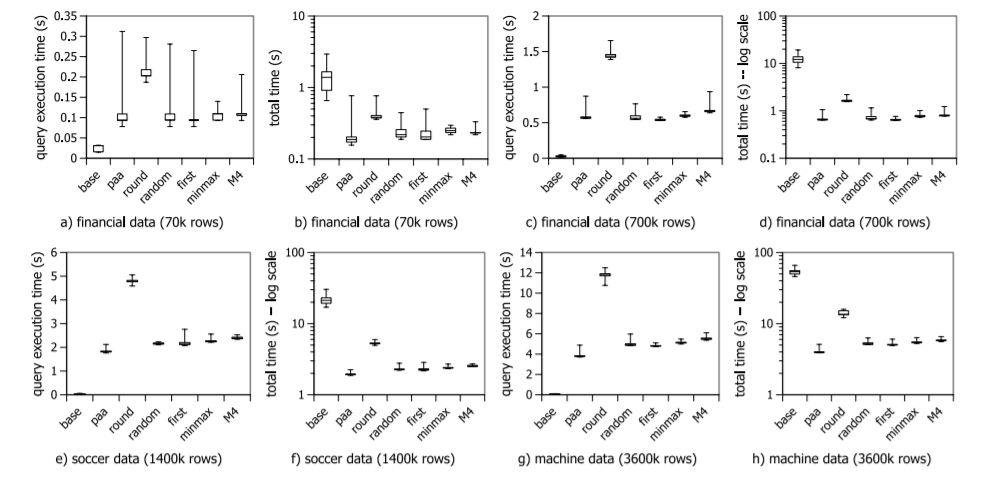
\includegraphics[width=\textwidth]{qp}
	\caption{Query performance: (a,b,c,d) financial data, (e,f) soccer data, (g,h) machine data}
	\label{qper}
\end{figure*}

\begin{figure*}
	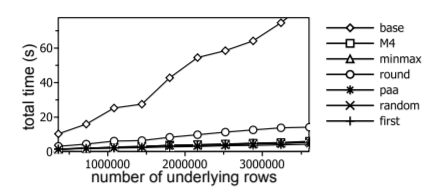
\includegraphics[width=0.5\textwidth]{pv}
	\caption{Performance of different queries with varying row counts}
	\label{vr}
\end{figure*}
\begin{figure*}
	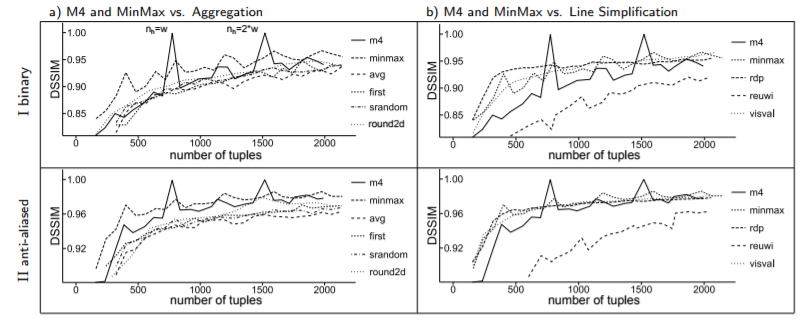
\includegraphics[width=\textwidth]{dsim}
	\caption{: Data efficiency of evaluated techniques, showing DSSIM over data volume}
	\label{dsim}
\end{figure*}

The query performance of different approaches in terms of execution time of the queries is shown in Figure \ref{qper}. It shows that aggregation based approaches perform better compared to baseline approaches. Figure \ref{vr} shows exemplary results of performance  for varying row counts on soccer data. The aggregation based queries perform much than baseline queries as the size of rows increase. 

\subsection{Visualization quality and Data Efficiency}
Authors in \cite{wang2004image} have shown that for visualization quality $MSE$ (Mean Square Error) doesn't perform well and they proposed $SSIM$ (Structural
Similarity Index) for the measurement of image quality. The SSIM yields a similarity
value between 1 and −1. The authors use $DSSIM$, the normalized distance between two visualizations for measuring the visualization quality. The formula is given below:
\begin{equation}
DSSIM(V_1, V_2) = \frac{1 - SSIM}{2}
\end{equation}

In Figure \ref{dsim}, the authors plotted the measured, resulting visualization
quality (DSSIM) over the resulting number of tuples of each
different groupings nh = 1 to nh = 2.5·w of an applied data
reduction technique. For readability, we cut off all low quality
results with DSSIM < 0.8. The lower the number of
tuples and the higher the DSSIM, the more data efficient is
the corresponding technique for the purpose of line visualization.
The Figures 14aI and 14bI depict these measures for
binary line visualizations and the Figures 14aII and 14bII
for anti-aliased line visualizations. We now observe the following
results.
